\section{实验四：双眼引导的双椭圆约束与低支持重建}\label{sec:lab4}

实验三的附加形态学补全表明，在单纯依赖 Cr/Cb 颜色阈值与最大连通域的框架下，$41\times41$ 无约束形态学补全只能在 $F1\approx70.7\%$ 的等值线上移动精确率—召回率工作点，无法突破“颜色与面积不包含人脸几何语义”的瓶颈。为在不引入预训练深度学习检测器的前提下突破这一上限，实验四在实验三的基础上按两个互补方向推进：其一是\textbf{尽量合并因阈值收紧或阴影而断裂的脸部碎片}（方向 A），其二是\textbf{尽量截断与脸部粘连的头发、脖颈和类肤色背景}（方向 B），并引入人脸椭圆几何先验统领两类操作。

由于 32 张测试图在实验三误差分析与形态学补全阶段已被逐张检视，实验四的全部探索、消融与参数选择均严格固定在 32 张验证集（开发集）上开展，以实验三初版方案在该集合上的表现（Precision 64.86\%、Recall 82.70\%、全局 F1 72.70\%、IoU 57.11\%）作为对照基线；验证集人工标签仅在预测掩膜与候选选择完全固定后用于事后评价。

\subsection{从最大连通域诊断到直接轮廓拟合的局限}

实验三在 $k=1.25$ 颜色阈值后直接保留最大 8 连通域并填孔。为量化“最大连通域筛选”究竟删去了什么，我们在 32 张验证图上对比了“原始阈值（\texttt{raw}）”“仅最大连通域（\texttt{largest}）”“跳过最大块直接填孔（\texttt{fill\_all}）”与“最大块后填孔（\texttt{largest\_fill}，即 Lab3 初版）”四个阶段，结果见表~\ref{tab:lab4_cc}。

\begin{table}[H]
\centering\small
\caption{验证集上最大连通域筛选与填孔的分阶段像素对照，指标单位为百分比}\label{tab:lab4_cc}
\begin{tabular}{lrrrrrr}
\toprule
阶段方案 & Precision & Recall & 全局 F1 & IoU & TP 像素数 & FP 像素数 \\
\midrule
原始阈值（$k=1.25$） & 52.43 & 60.39 & 56.13 & 39.01 & 1,345,567 & 1,220,918 \\
仅保留最大连通域 & 59.23 & 57.61 & 58.41 & 41.25 & 1,283,698 & 883,679 \\
跳过最大块直接填孔 & 58.34 & 84.71 & 69.10 & 52.78 & 1,887,542 & 1,347,802 \\
最大连通域加填孔（Lab3） & 64.86 & 82.70 & 72.70 & 57.11 & 1,842,674 & 998,367 \\
\bottomrule
\end{tabular}
\end{table}

数据显示，在填孔前直接取最大连通域虽然去除了 337,239 个非脸误检像素，但也永久删去了 61,869 个真实脸部像素；反之，若跳过最大连通域直接填孔，虽然找回了更多脸部像素（Recall 达 84.71\%），却保留了 1,347,802 个误检像素，且在脸部外轮廓未闭合的样本上依然无法靠填孔恢复内部。图~\ref{fig:lab4_cc_00562} 展示了验证集困难样本 00562 的分阶段差异：原始阈值下脸部碎裂为额头、鼻梁、嘴唇等互不相连的小块，而外围发际与脖颈构成了最大连通域；取最大连通域后，橙色标出的内脸正确碎片被悉数删去，后续填孔也因轮廓敞开而完全失效（Lab3 F1 仅为 0.1295）。

\begin{figure}[H]
\centering
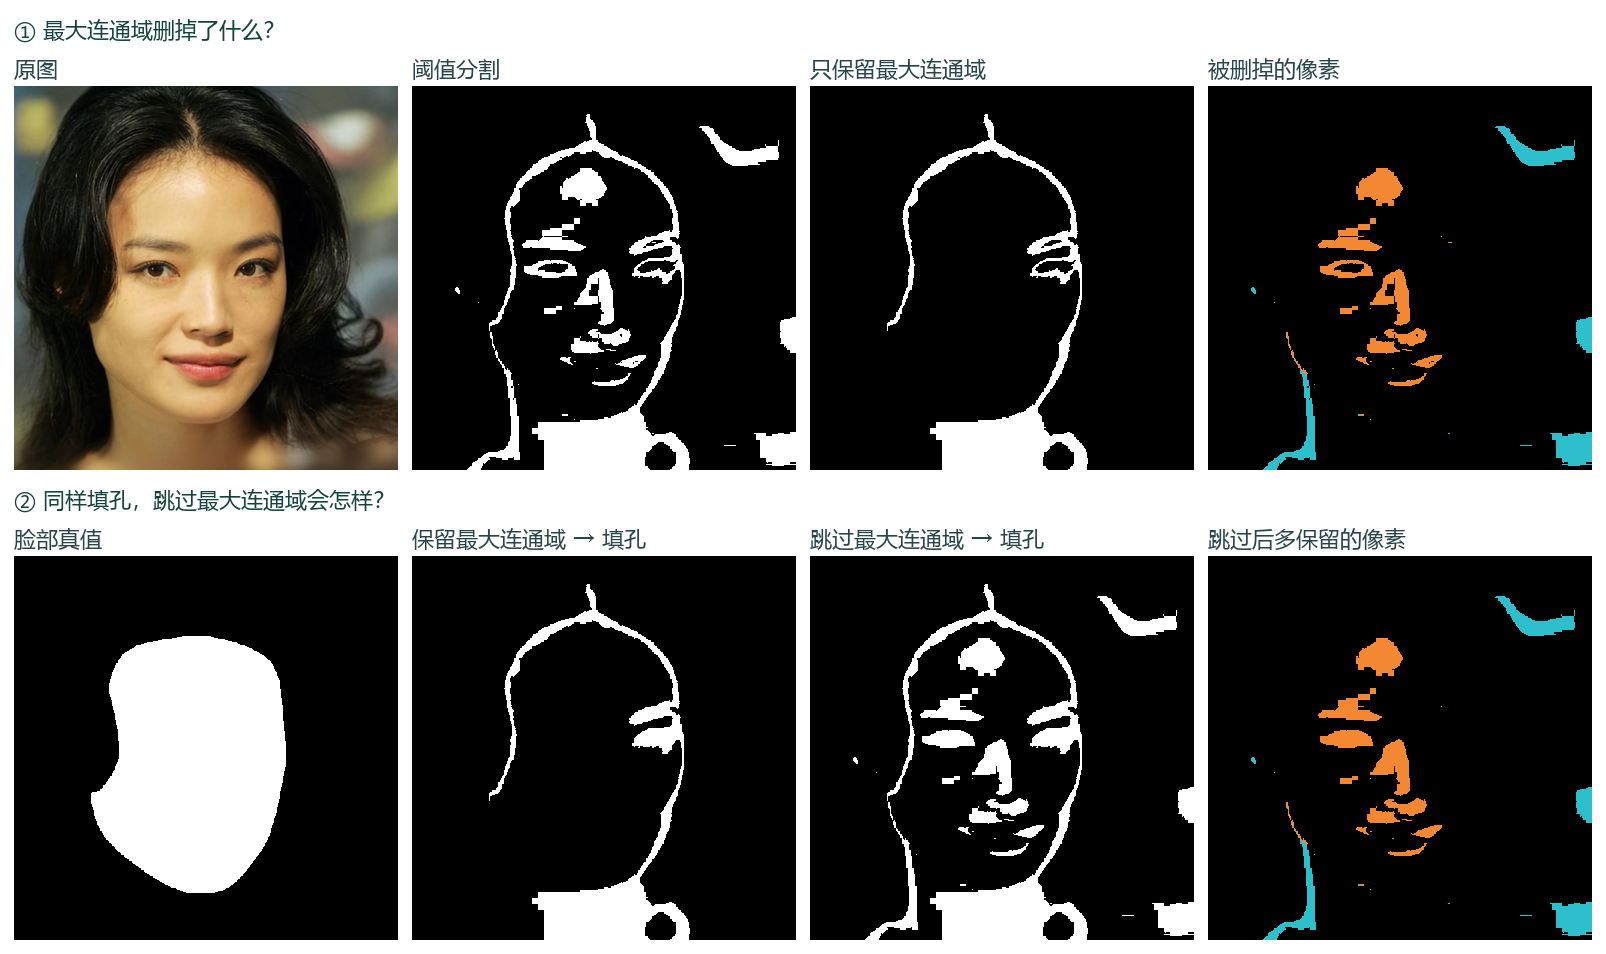
\includegraphics[width=0.96\textwidth]{lab4_cc_00562.png}
\caption{验证图 00562 的最大连通域分阶段诊断。上排右图橙色为最大连通域筛选误删的真实脸部碎片，青色为正确排除的背景；下排显示无论是否保留最大连通域，敞口轮廓均无法靠普通填孔恢复内脸。}
\label{fig:lab4_cc_00562}
\end{figure}

基于经典人脸椭圆几何模型\cite{wang1999frontal,garcia1999face}，我们首先尝试直接从肤色候选轮廓拟合人脸椭圆：对原始阈值、$5\times5$ 椭圆核闭运算（轻量连接）和 $5\times5$ 椭圆核开运算（轻量分离）三种输入，分别提取连通块与近邻组合，调用 OpenCV \texttt{fitEllipse} 拟合外轮廓点，并以同心缩放的内椭圆（$0.8$ 倍轴长）做 $9\times9$ 闭运算修补、外椭圆（$1.15$ 倍轴长）裁剪外围误检。表~\ref{tab:lab4_weak_refine} 给出了 32 张验证图上各来源默认最大候选的一轮修整结果。

\begin{table}[H]
\centering\footnotesize
\setlength{\tabcolsep}{4pt}
\caption{弱形态学预操作与直接肤色轮廓椭圆修整的验证集对比，单位为百分比}\label{tab:lab4_weak_refine}
\begin{tabular}{lrrrrrr}
\toprule
候选来源 & 外椭圆 F1 & 修整后 P & 修整后 R & 修整后 F1 & 修整后 IoU & 相对 Lab3 $\Delta$F1 \\
\midrule
Lab3 基线（最大块填孔） & -- & 64.86 & 82.70 & 72.70 & 57.11 & 0.00 \\
原始阈值轮廓椭圆 & 60.06 & 65.66 & 81.96 & 72.91 & 57.37 & +0.21 \\
$5\times5$ 闭运算轮廓椭圆 & 59.69 & 64.71 & 82.22 & 72.42 & 56.77 & $-0.28$ \\
$5\times5$ 开运算轮廓椭圆 & 59.02 & 65.32 & 67.76 & 66.52 & 49.83 & $-6.18$ \\
\bottomrule
\end{tabular}
\end{table}

这一轮探索给出了明确的否定性结论：第一，$5\times5$ 闭运算无法跨过较大尺度的面部阴影断裂，修整后 F1（72.42\%）反而略低于 Lab3；第二，$5\times5$ 开运算在切断背景细桥的同时严重削弱了原本有用的脸部边缘，导致 Recall 跌至 67.76\%、F1 降至 66.52\%；第三，直接对肤色轮廓拟合椭圆仅比 Lab3 高 0.21 个百分点，原因在于\textbf{当头发或脖颈与脸部粘连时，外轮廓拟合出的椭圆会被错误区域带偏；当脸部严重碎裂时，局部碎片又只能拟合出偏小椭圆}。这说明椭圆的位置、尺度和方向不能依赖待修整的肤色轮廓本身，必须引入独立于肤色连通块的五官定位锚点。

\subsection{双眼位置识别：灰度黑帽变换与双窗空间先验}

实验三在转换至 YCrCb 后丢弃了亮度通道 $Y$，导致深色头发与阴影皮肤在色度上难以区分；但从五官结构看，双眼在灰度图 $I_{\text{gray}}$ 中呈现稳定的局部暗斑与水平成对几何关系\cite{hsu2002face}。受此启发，我们在不使用任何预训练人脸或眼睛检测器的前提下，利用灰度形态学\textbf{黑帽变换（Black-Hat Transform）}提取局部暗部响应：
\begin{equation}
R_{\text{bh}}(x,y) = \bigl((I_{\text{gray}} * G_{3\times3}) \bullet B_{\text{bh}}\bigr)(x,y) - (I_{\text{gray}} * G_{3\times3})(x,y),
\label{eq:blackhat}
\end{equation}
其中 $G_{3\times3}$ 为高斯平滑核，$\bullet$ 表示形态学闭运算，$B_{\text{bh}}$ 为横向椭圆形结构元素（宽高取粗略面宽尺度 $W_s$ 的 $13\%$ 与 $7\%$ 并取奇数）。黑帽响应经 $\max(12, T_{\text{Otsu}})$ 阈值化与 $1\times3$ 横向闭运算后，按连通域宽高、面积与长宽比 $[0.65, 7.0]$ 筛选暗部候选，再按眼距范围 $[0.18W_s, 0.65W_s]$、连线倾角 $|\theta|\le 25^\circ$ 及左右候选面积比 $r_{\text{area}}=\min(A_L,A_R)/\max(A_L,A_R)$ 进行配对。每对候选的图像视觉基础分 $S_{\text{base}}$ 由五项归一化特征加权组成：
\begin{equation}
S_{\text{base}} = 0.25\,S_{\text{align}} + 0.15\,r_{\text{area}} + 0.15\,S_{\text{space}} + 0.25\,S_{\text{resp}} + 0.20\,S_{\text{skin}},
\label{eq:eyebase}
\end{equation}
分别衡量水平对齐度 $1-|\theta|/25^\circ$、双斑面积相近度、间距接近 $0.36W_s$ 的程度、黑帽响应强度均值，以及候选外围环形邻域内的原始肤色支持率。

为检验图像暗部特征与空间先验各自的贡献，我们在 32 张验证图上依次推进了三轮定位实验。训练集 98 张图像中有 97 张包含完整双眼标注（标签 4、5，样本 00615 除外）；仅用这 97 张训练图统计归一化左眼中心 $\boldsymbol{\mu}_L=(0.3778, 0.4769)$、右眼中心 $\boldsymbol{\mu}_R=(0.6198, 0.4756)$。由于训练集实测标准差极小（约 $0.005\text{--}0.009$），我们将两眼标准差下限放宽至 $\boldsymbol{\sigma}_L=\boldsymbol{\sigma}_R=(0.025, 0.018)$，在第三轮中以 $3\sigma$ 椭圆窗口（对 $512\times512$ 图像半轴约为 $38.4\times27.6$ 像素）分别限制左右眼搜索范围，不再依赖可能出错的肤色连通块外接框，并以训练集平均眼距的 $2.5$ 倍作为统一面宽尺度 $W_s$。记左、右眼候选中心到各自训练均值的标准化平方距离为
\begin{equation}
d_i^2 = \left(\frac{x_i/W - \mu_{i,x}}{\sigma_{i,x}}\right)^2 + \left(\frac{y_i/H - \mu_{i,y}}{\sigma_{i,y}}\right)^2, \qquad i\in\{L,R\},
\label{eq:eyedist}
\end{equation}
则双窗位置得分为两眼高斯得分的几何均值 $S_{\text{pos}}=\exp\bigl(-(d_L^2+d_R^2)/4\bigr)$，综合配对得分为
\begin{equation}
S_{\text{pair}} = (1 - w_p)S_{\text{base}} + w_p S_{\text{pos}}, \qquad w_p = 0.65.
\label{eq:eyepairscore}
\end{equation}
以标签双眼质心为事后评价参考，定义归一化定位误差 $e = \max\bigl(\|\hat{\mathbf{p}}_L-\mathbf{p}_L\|_2, \|\hat{\mathbf{p}}_R-\mathbf{p}_R\|_2\bigr) / \|\mathbf{p}_R-\mathbf{p}_L\|_2$，三轮定位结果及“完全不看图像、直接输出训练均值”的诊断对照汇总于表~\ref{tab:lab4_eyes}。

\begin{table}[H]
\centering\footnotesize
\setlength{\tabcolsep}{4pt}
\caption{验证集 32 张图像上的双眼定位准确率演进与均值诊断对照}\label{tab:lab4_eyes}
\begin{tabular}{lrrrr}
\toprule
定位方法 & 配对数 & 首选 $e\le 0.15$ & 首选 $e\le 0.25$ & 中位误差 $e$ \\
\midrule
第一轮：无位置先验（肤色框内搜索） & 30/32 & 13/32（40.6\%） & 13/32（40.6\%） & 0.2648 \\
第二轮：双眼中点弱先验（$w_p=0.20$） & 30/32 & 15/32（46.9\%） & 15/32（46.9\%） & 0.1876 \\
第三轮：两眼独立窗口约束（$w_p=0.65$） & 29/32 & 26/32（81.3\%） & 28/32（87.5\%） & 0.0466 \\
诊断对照：仅输出训练集双眼均值 & 32/32 & 32/32（100.0\%） & 32/32（100.0\%） & 0.0569 \\
\bottomrule
\end{tabular}
\end{table}

表~\ref{tab:lab4_eyes} 揭示了两个关键事实。第一，无位置先验时，仅靠“水平成对暗部”极易将双眉（如 00590，$e=0.265$）或发丝空隙（如 00690，$e=2.749$）排在真实双眼之前；引入两眼独立搜索窗与位置加权后，$e\le 0.25$ 合格率从 40.6\% 跃升至 87.5\%，中位误差降至 0.0466（见图~\ref{fig:lab4_eye_00590}）。第二，诊断对照表明，直接输出训练均值在当前验证集上即可达到 32/32 合格，说明本数据集人像构图高度居中对齐；因此双眼定位的高准确率在很大程度上受益于数据集构图一致性。

\begin{figure}[H]
\centering
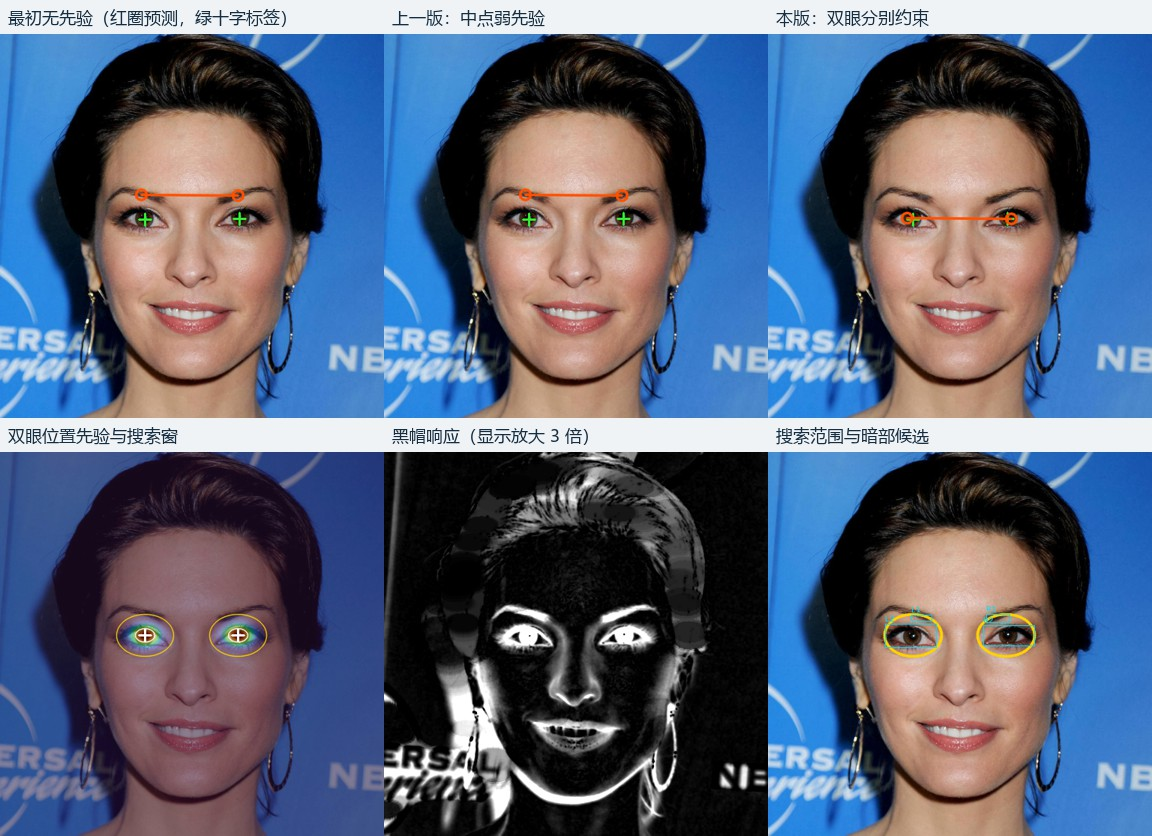
\includegraphics[width=0.96\textwidth]{lab4_eye_00590.jpg}
\caption{验证图 00590 的三版双眼定位对比与中间响应。无先验与中点弱先验均误选双眉（红圈偏离绿十字真值），双窗约束结合灰度黑帽响应准确锁定双眼。}
\label{fig:lab4_eye_00590}
\end{figure}

此外，第三轮严格配对规则（$r_{\text{area}}\ge 0.30$）在 00655 与 00690 上因单侧眼部受刘海或阴影影响、左右暗斑面积比约为 0.275 而未能输出配对。为此，我们在最终流程中设计了\textbf{严格优先、放宽回退}的两级配对机制：优先采用 $r_{\text{area}}\ge 0.30$ 的严格配对（\texttt{standard\_pair}，覆盖 29 张）；仅当严格配对为空时，才回退至 $r_{\text{area}}\ge 0.20$ 的放宽配对（\texttt{recovered\_pair}，成功找回 00655 与 00690）；若仍无配对（仅 00592 一张），则安全回退至 Lab3 掩膜（\texttt{no\_pair}），绝不盲目填入训练统计均值。

\subsection{双椭圆空间约束与侧向姿态候选}

确定双眼中心 $\mathbf{p}_L, \mathbf{p}_R$ 后，即可脱离容易受头发干扰的肤色轮廓，在以双眼为基准的局部坐标系下直接推算人脸椭圆。定义双眼中点 $\mathbf{m}=(\mathbf{p}_L+\mathbf{p}_R)/2$、眼距 $d_{\text{eye}}=\|\mathbf{p}_R-\mathbf{p}_L\|_2$、眼线单位向量 $\mathbf{u}=(\mathbf{p}_R-\mathbf{p}_L)/d_{\text{eye}}$，以及朝向面部下方的正交法向量 $\mathbf{v}=(-u_y, u_x)^\top$（取 $v_y\ge 0$）。在 97 张有效训练图上，对脸部真值最大连通块拟合椭圆并投影至 $(\mathbf{m}, \mathbf{u}, \mathbf{v}, d_{\text{eye}})$ 坐标系，按分量取中位数得到固定的五参数几何先验：
\begin{equation}
\alpha_\parallel = 0.0159,\quad
\alpha_\perp = 0.3986,\quad
\gamma_{\text{major}} = 2.8942,\quad
\gamma_{\text{minor}} = 2.1489,\quad
\Delta\theta = -0.7843^\circ.
\label{eq:geomprior}
\end{equation}
由此，任意检测到双眼的图像可生成正中基础椭圆 $E_{\text{base}}$：中心 $\mathbf{c}_0 = \mathbf{m} + d_{\text{eye}}(\alpha_\parallel\mathbf{u} + \alpha_\perp\mathbf{v})$，长短轴直径 $(2a_0, 2b_0) = d_{\text{eye}}(\gamma_{\text{major}}, \gamma_{\text{minor}})$，主轴倾角 $\theta_0 = \operatorname{atan2}(v_y, v_x) + \Delta\theta$。仅将 $E_{\text{base}}$ 直接光栅化为二值掩膜（不结合任何肤色分割），在 29 张严格检出双眼的验证图上即可取得全局 F1 81.88\%（图~\ref{fig:lab4_eye_ellipse_00535}），证实了眼睛锚点对人脸尺度和中心定位的稳定性。

\begin{figure}[H]
\centering
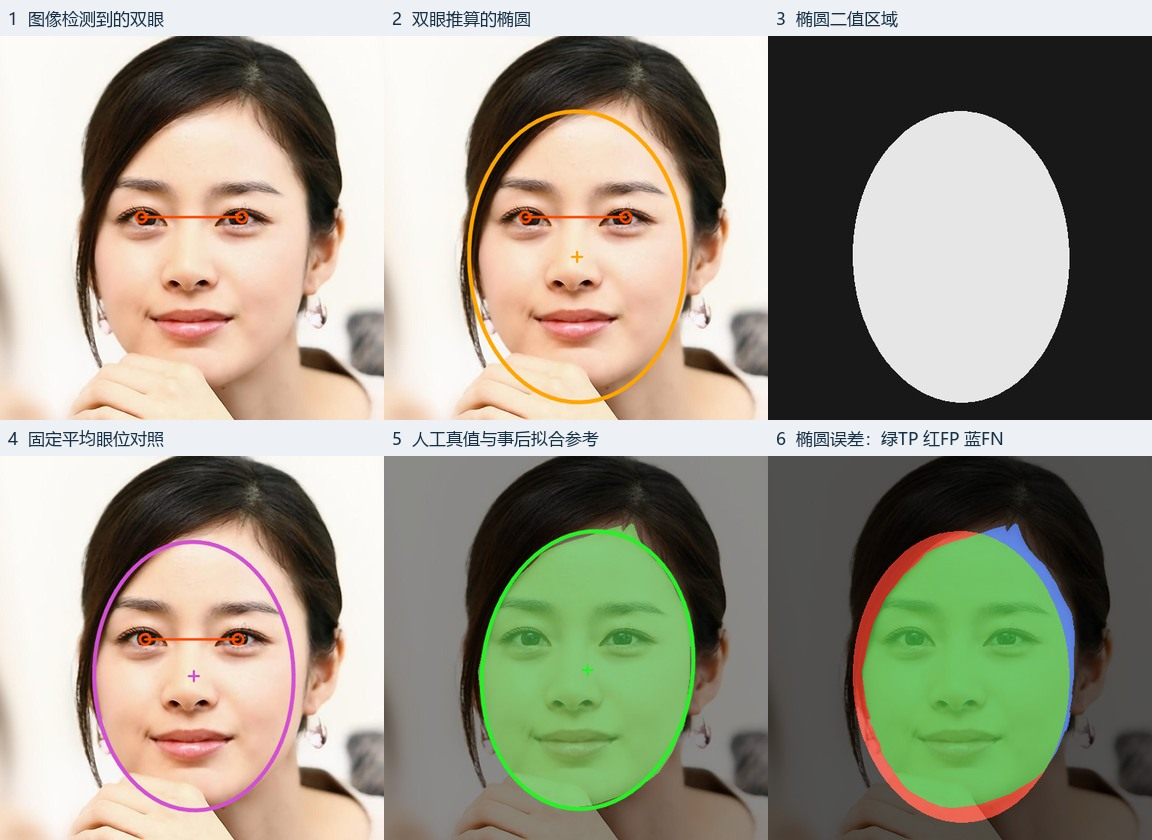
\includegraphics[width=0.96\textwidth]{lab4_eye_ellipse_00535.jpg}
\caption{验证图 00535 由双眼推算正中脸部椭圆的过程对照。双眼距离与倾角直接决定椭圆中心、长短轴与朝向，无需依赖易受背景污染的肤色外轮廓。}
\label{fig:lab4_eye_ellipse_00535}
\end{figure}

在此基础上，我们进一步引入两项空间结构设计：
\begin{enumerate}
\item \textbf{针对侧脸与偏转姿态的侧向椭圆候选：}当人脸发生左右偏转（侧脸或四分之三侧面）时，由于透视缩短效应，双眼中点会偏向朝向镜头的一侧，而另一侧脸颊与下颌占画面更宽。为此，沿眼线方向 $\mathbf{u}$ 按眼距比例 $s\in\{0, -0.16, +0.16\}$ 平移椭圆中心，构造正中（\texttt{center}）、画面左偏（\texttt{image\_left}）和画面右偏（\texttt{image\_right}）三个姿态候选：
\begin{equation}
\mathbf{c}_s = \mathbf{c}_0 + s \cdot d_{\text{eye}}\mathbf{u}, \qquad s \in \{0,\; -0.16,\; +0.16\}.
\label{eq:poseshift}
\end{equation}
\item \textbf{内外嵌套双椭圆分区约束：}椭圆的作用不是直接替代人脸掩膜，而是为形态学处理划定空间边界。对每个姿态候选，保持中心 $\mathbf{c}_s$ 与倾角 $\theta_0$ 不变，按比例 $\lambda_{\text{in}}=0.82$ 与 $\lambda_{\text{out}}=1.20$ 缩放长短轴，生成\textbf{内椭圆 $E_{\text{in}}$} 与\textbf{外椭圆 $E_{\text{out}}$}（满足 $E_{\text{in}}\subset E_{\text{out}}$）：
\begin{itemize}
\item \textbf{核心区 $E_{\text{in}}$：}代表高置信度面部内部，提取核心种子并允许较强形态学闭运算、填孔及低支持重建；
\item \textbf{过渡环带 $E_{\text{out}}\setminus E_{\text{in}}$：}包含发际线、脸颊边缘与下颌轮廓，仅允许小尺度弱闭运算修补细缝，优先保留原有颜色边界证据；
\item \textbf{外部抑制区 $\overline{E_{\text{out}}}$：}直接截断延伸至外椭圆之外的头发、脖颈与背景粘连块，严禁任何形态学扩张越界。
\end{itemize}
\end{enumerate}

为在不接触真值标签的前提下自动选择姿态候选，我们定义无监督图像支持度评分 $S_{\text{cand}}$：
\begin{equation}
S_{\text{cand}} = 0.55\,\rho_{\text{in}} + 0.20\,\rho_{\text{out}} + 0.20\,r_{\text{ret}} - 0.15\,\rho_{\partial E_{\text{out}}},
\label{eq:candscore}
\end{equation}
其中 $\rho_{\text{in}} = |M_{\text{sel}}\cap E_{\text{in}}|/|E_{\text{in}}|$ 与 $\rho_{\text{out}} = |M_{\text{sel}}\cap E_{\text{out}}|/|E_{\text{out}}|$ 分别为内、外椭圆内的肤色支持率，$r_{\text{ret}} = |M_{\text{sel}}|/|M_{\text{local}}|$ 为外椭圆内保留的核心连通域比例，$\rho_{\partial E_{\text{out}}}$ 为最终掩膜在外椭圆 $3\times3$ 腐蚀边界带上的占据率。同时，对侧向候选施加优势门槛 $\Delta S_{\text{lat}}=0.06$，防止近似正脸因局部头发干扰产生无益偏移。

\subsection{低支持度放宽肤色阈值重选与分区形态学连接}

双椭圆外边界裁剪有效解决了“背景与头发粘连”问题，但对于光照偏暗或严重偏色的样本（如 00548、00562、00660、00733），实验三在 $k=1.25$ 下的掩膜 $M_{\text{Lab3}}$ 落入内椭圆 $E_{\text{in}}$ 的像素极少，即便在 $E_{\text{in}}$ 内执行常规闭运算也无从连接。

针对这一“内椭圆像素过少”的失效模式，我们设计了\textbf{低支持度放宽阈值受限重建机制}：
\begin{enumerate}
\item \textbf{核心种子提取与低支持判别：}取外椭圆裁剪后的初始掩膜 $M_{\text{local}} = M_{\text{Lab3}} \cap E_{\text{out}}$，仅保留其中与内椭圆 $E_{\text{in}}$ 交集不少于 $N_{\text{core}}=24$ 像素的 8 连通分量，记为 $M_{\text{sel}}$，其内椭圆部分 $S = M_{\text{sel}} \cap E_{\text{in}}$ 作为高可信核心种子。计算内椭圆支持率 $\rho_{\text{in}} = |S| / |E_{\text{in}}|$；当 $\rho_{\text{in}} < \tau_{\text{low}} = 0.18$ 时，判定为低支持度样本。
\item \textbf{放宽肤色阈值重选与内椭圆形态学重建：}当阈值系数从 $k=1.25$ 放宽至 $k_{\text{rec}}=2.00$ 时，训练集肤色覆盖率可提升至 91.86\%。在全图放宽会引发灾难性背景误检，但在内椭圆 $E_{\text{in}}$ 内部放宽则是安全的。因此，仅在低支持样本的 $E_{\text{in}}$ 内启用 $k_{\text{rec}}=2.00$ 的放宽肤色掩膜 $M_{\text{relax}}$，以 $27\times27$ 椭圆核执行闭运算连接面部碎片，并严格只保留与高可信种子 $S$ 重叠不少于 24 像素的连通分量，填孔后得到受限重建区域 $M_{\text{rec}}$：
\begin{equation}
\begin{aligned}
A &= \bigl(\operatorname{Close}_{27}(M_{\text{relax}}\cap E_{\text{in}})\cap E_{\text{in}}\bigr)\cup S,\\
M_{\text{rec}} &= \operatorname{FillHoles}\!\left(\bigcup_{C_j\in\mathcal{C}_8(A):\,|C_j\cap S|\ge 24} C_j\right)\cap E_{\text{in}}.
\end{aligned}
\label{eq:lowsupport}
\end{equation}
\item \textbf{分区形态学连接与种子锚定输出：}内椭圆核心区采用 $11\times11$ 强闭运算与填孔（低支持样本并入 $M_{\text{rec}}$），过渡环带 $E_{\text{out}}\setminus E_{\text{in}}$ 采用 $5\times5$ 弱闭运算；两者合并为候选掩膜 $M_{\text{prop}}$ 后，再次按 8 连通提取与核心种子 $S$ 相交的连通块并做最终填孔：
\begin{equation}
\begin{aligned}
M_{\text{prop}} &= \Bigl(\bigl(\operatorname{FillHoles}(\operatorname{Close}_{11}(M_{\text{sel}}))\cap E_{\text{in}}\bigr)\cup M_{\text{rec}}\Bigr)
\;\cup\; \Bigl(\operatorname{Close}_{5}(M_{\text{sel}})\cap (E_{\text{out}}\setminus E_{\text{in}})\Bigr),\\
M_{\text{final}} &= \operatorname{FillHoles}\!\left(\bigcup_{C_j\in\mathcal{C}_8(M_{\text{prop}}):\,C_j\cap S\neq\emptyset} C_j\right)\cap E_{\text{out}}.
\end{aligned}
\label{eq:zonalmorph}
\end{equation}
\end{enumerate}

\subsection{验证集消融实验与整体指标提升}

我们在 32 张验证图上对侧向椭圆门槛、低支持度放宽阈值系数 $k_{\text{rec}}$ 与连接核大小进行了系统消融，完整演进记录见表~\ref{tab:lab4_ablation}。

\begin{table}[H]
\centering\footnotesize
\setlength{\tabcolsep}{3pt}
\caption{验证集（32 张）从实验三到实验四各阶段的消融与优化结果，指标单位为百分比}\label{tab:lab4_ablation}
\begin{tabular}{lrrrrrr}
\toprule
方案与实验阶段 & P & R & 全局 F1 & IoU & 均值 F1 & 升/降/平 \\
\midrule
原始颜色阈值（$k=1.25$） & 52.43 & 60.39 & 56.13 & 39.01 & 54.92 & -- \\
Lab3 初版（最大连通域 + 填孔） & 64.86 & 82.70 & 72.70 & 57.11 & 70.67 & 对照基线 \\
Lab3 形态学补全（$41\times41$ 膨胀填孔腐蚀） & 61.77 & 86.22 & 71.98 & 56.22 & 71.50 & 19/13/0 \\
Lab4 肤色轮廓椭圆一轮修整（无眼睛定位） & 65.66 & 81.96 & 72.91 & 57.37 & 71.75 & -- \\
Lab4 双椭圆基线（$\Delta S_{\text{lat}}=0.04$，无重建） & 79.48 & 80.06 & 79.77 & 66.35 & 75.69 & 28/3/1 \\
试验 1：侧向门槛 $\Delta S_{\text{lat}}=0.06$（无重建） & 79.67 & 80.01 & 79.84 & 66.45 & 75.75 & 28/3/1 \\
试验 2A：低支持重建（$\rho_{\text{in}}<0.18, k=1.55$, 核 15） & -- & -- & 81.24 & 68.41 & -- & 29/2/1 \\
试验 2B：低支持重建（$\rho_{\text{in}}<0.18, k=1.75$, 核 21） & -- & -- & 82.27 & 69.87 & 81.22 & 29/2/1 \\
\textbf{试验 2C（最终采用）：低支持重建（$k=2.00$, 核 27）} & \textbf{79.88} & \textbf{86.15} & \textbf{82.89} & \textbf{70.79} & \textbf{82.19} & \textbf{29/2/1} \\
试验 2D（过强，未采用）：低支持重建（$k=2.25$, 核 33） & -- & -- & 83.50 & -- & -- & 趋近填满 \\
事后理想姿态上界（Oracle 选正中/左偏/右偏） & 81.18 & 87.97 & 84.44 & 73.07 & 83.75 & 诊断上界 \\
\bottomrule
\end{tabular}
\end{table}

消融过程清晰展示了每一步优化的作用与取舍边界：
\begin{enumerate}
\item \textbf{双椭圆空间约束打破等值线权衡：}引入双眼定位与内外椭圆分区形态学后，即便尚未加入低支持重建（试验 1），验证集 Precision 已从 Lab3 的 64.86\% 大幅跃升至 79.67\%（+14.81 个百分点），FP 像素从 998,367 锐减至 454,790（减少 54.45\%），全局 F1 从 72.70\% 提升至 79.84\%。
\item \textbf{侧向椭圆门槛控制与姿态潜力：}在基线 $\Delta S_{\text{lat}}=0.04$ 下，有 3 张图像自动选择了侧向椭圆，但事后核查发现这 3 次偏移均由发丝不对称引起，并未优于正中椭圆。将门槛提高至 $\Delta S_{\text{lat}}=0.06$ 后，31 张检出双眼的图像全部稳健保留正中椭圆，全局 F1 微升至 79.84\%。与此同时，若能为每张图准确选取正中/左偏/右偏三者中的最优姿态（Oracle 上界，其中 16 张左偏最优、10 张右偏最优、5 张正中最优），全局 F1 可进一步达 84.44\%、IoU 达 73.07\%，说明侧向椭圆候选机制本身对偏转人脸确有约 1.55 个百分点的额外空间。
\item \textbf{低支持度放宽阈值重建显著拉升召回率与均值 F1：}在 $\rho_{\text{in}}<0.18$ 触发条件下（共触发 00548、00562、00660、00733 四张困难样本），随着 $(k_{\text{rec}}, \text{核大小})$ 从 $(1.55, 15)$ 增至 $(2.00, 27)$，验证集 Recall 从无重建时的 80.01\% 回升至 86.15\%（高于 Lab3 的 82.70\%），全局 F1 达到 \textbf{82.89\%}（比 Lab3 提升 \textbf{+10.19 个百分点}），IoU 达到 \textbf{70.79\%}（比 Lab3 提升 \textbf{+13.68 个百分点}），逐图平均 F1 更从 70.67\% 提升至 82.19\%（+11.52 个百分点）。当继续增大到试验 2D 的 $(2.25, 33)$ 时，4 张低支持图的重建结果已逼近直接填满整个内椭圆，额头上方黑发误填风险显著上升，故最终定型于试验 2C（$k_{\text{rec}}=2.00$，连接核 27）。
\end{enumerate}

\subsection{典型案例分析与方法边界}

表~\ref{tab:lab4_cases} 列出了验证集上触发低支持重建的 4 张困难样本，以及背景粘连裁剪、放宽配对恢复、无双眼回退和轻微退步的代表性样本指标对比。

\begin{table}[H]
\centering\small
\setlength{\tabcolsep}{3.5pt}
\caption{验证集典型样本在 Lab3 与 Lab4 最终方案下的像素变化与指标对照}\label{tab:lab4_cases}
\begin{tabular}{llrrrrrrr}
\toprule
样本编号 & 运行机制分支 & Lab3 P & Lab4 P & Lab3 R & Lab4 R & Lab3 F1 & Lab4 F1 & $\Delta$F1 \\
\midrule
00548 & 严格配对 + 低支持重建 & 39.51 & 57.77 & 9.01 & 47.26 & 14.68 & 51.99 & +37.31 \\
00562 & 严格配对 + 低支持重建 & 29.12 & 77.21 & 8.33 & 69.39 & 12.95 & 73.09 & +60.14 \\
00660 & 严格配对 + 低支持重建 & 38.65 & 73.33 & 14.08 & 88.74 & 20.64 & 80.31 & +59.67 \\
00733 & 严格配对 + 低支持重建 & 8.40 & 53.92 & 9.01 & 66.35 & 8.69 & 59.49 & +50.80 \\
00611 & 严格配对 + 双椭圆裁剪 & 32.91 & 51.11 & 100.00 & 100.00 & 49.52 & 67.64 & +18.12 \\
00632 & 严格配对 + 双椭圆裁剪 & 53.96 & 86.19 & 97.59 & 77.38 & 69.50 & 81.55 & +12.05 \\
00655 & 放宽眼面积比恢复配对 & 82.31 & 95.69 & 66.86 & 66.22 & 73.78 & 78.27 & +4.49 \\
00690 & 放宽眼面积比恢复配对 & 61.14 & 74.85 & 99.71 & 80.98 & 75.80 & 77.80 & +2.00 \\
00592 & 无双眼配对安全回退 & 80.96 & 80.96 & 93.92 & 93.92 & 86.96 & 86.96 & 0.00 \\
00712 & 轻微退步（外椭圆边际） & 79.46 & 79.14 & 99.88 & 99.90 & 88.51 & 88.32 & $-0.19$ \\
00731 & 轻微退步（外椭圆边际） & 92.35 & 92.15 & 99.72 & 99.73 & 95.89 & 95.79 & $-0.10$ \\
\bottomrule
\end{tabular}
\end{table}

结合具体图像可以清楚看到两类核心机制的作用方式：
\begin{itemize}
\item \textbf{外椭圆抑制大面积背景与头发粘连（方向 B）：}在图~\ref{fig:lab4_dual_00632}（样本 00632）中，人物呈微侧脸姿态，棕色长发、脖颈与背景在 $k=1.25$ 下与脸部连成覆盖大半幅画面的单一连通块，Lab3 精确率仅为 53.96\%（F1 为 0.6950）。Lab4 由双眼定出内外椭圆后，外椭圆一次性裁剪掉 74,165 个外部误检像素，使精确率跃升至 86.19\%，F1 提高至 0.8155。
\item \textbf{低支持放宽阈值重建找回碎裂与缺失内脸（方向 A）：}在图~\ref{fig:lab4_dual_00562}（样本 00562）与图~\ref{fig:lab4_dual_00660}（样本 00660）中，Lab3 因阴影或偏色导致内脸大面积镂空甚至只选中右下颌与脖子（Recall 仅 8.33\% 与 14.08\%）。由于内椭圆支持率 $\rho_{\text{in}}<0.18$，算法自动触发 $k_{\text{rec}}=2.00$ 放宽肤色重选与 $27\times27$ 闭运算受限重建：00562 补回 42,481 个真实脸部像素而仅新增 720 个误检像素，F1 从 0.1295 跃升至 0.7309（+0.6014）；00660 补回 38,240 个真实脸部像素，F1 从 0.2064 跃升至 0.8031（+0.5967）。
\end{itemize}

\begin{figure}[H]
\centering
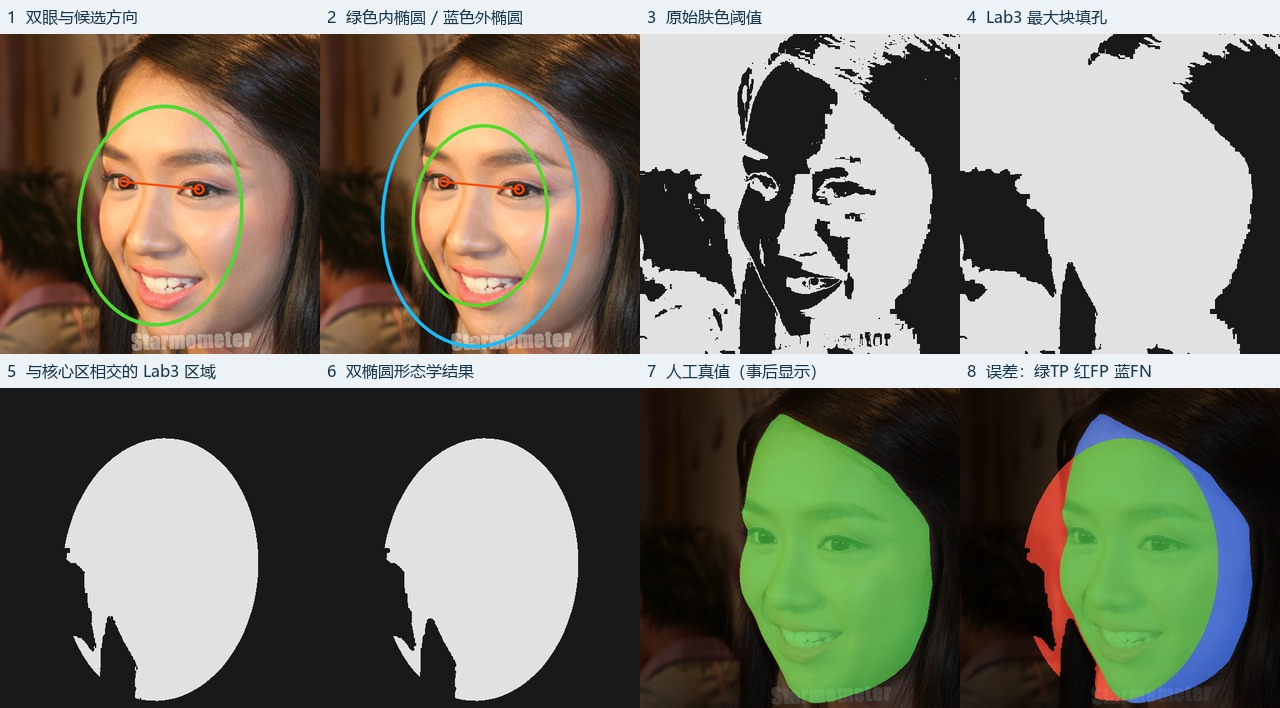
\includegraphics[width=0.98\textwidth]{lab4_dual_00632.jpg}
\caption{验证图 00632 的双椭圆约束形态学全流程对照。外椭圆有效截断了与脸部粘连的大片头发与背景（去除 74,165 个 FP 像素），F1 从 0.6950 提升至 0.8155。}
\label{fig:lab4_dual_00632}
\end{figure}

\begin{figure}[H]
\centering
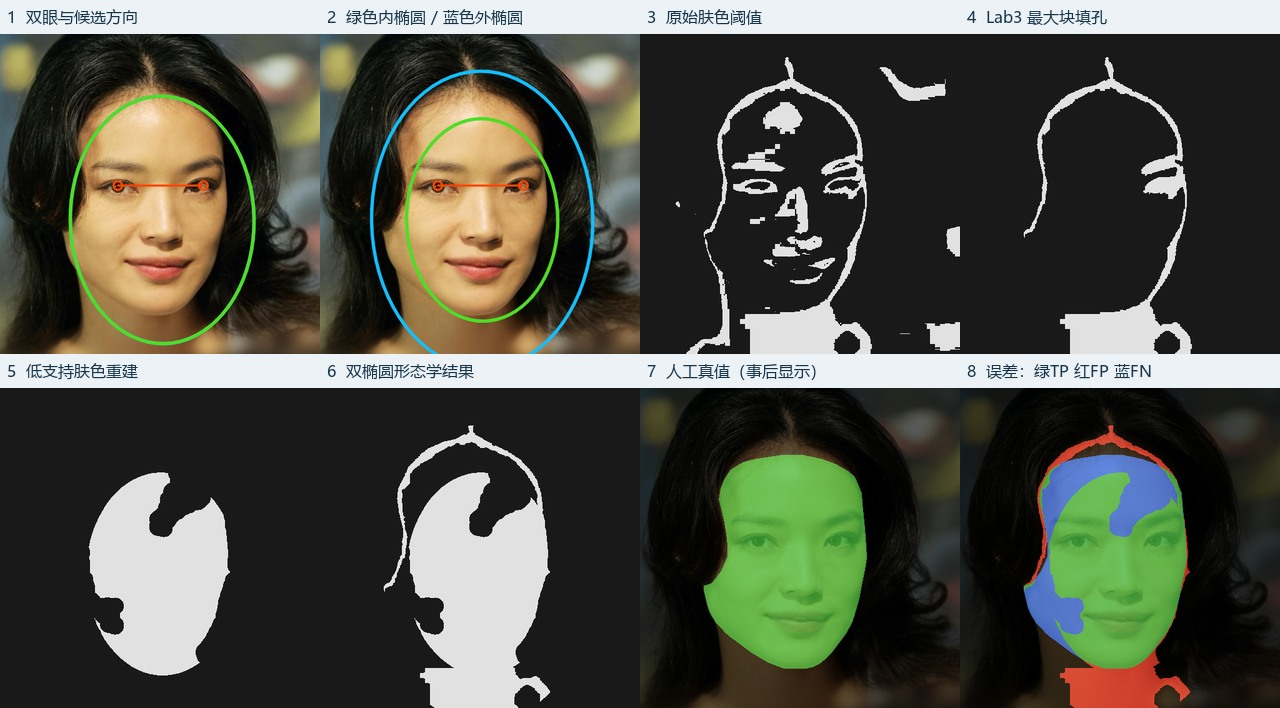
\includegraphics[width=0.98\textwidth]{lab4_dual_00562.jpg}
\caption{验证图 00562 的低支持度放宽阈值重建对照。内椭圆支持率低于 0.18 触发 $k=2.00$ 放宽肤色重选与 27 像素闭运算连接，在核心区内恢复整张内脸，F1 从 0.1295 提升至 0.7309。}
\label{fig:lab4_dual_00562}
\end{figure}

\begin{figure}[H]
\centering
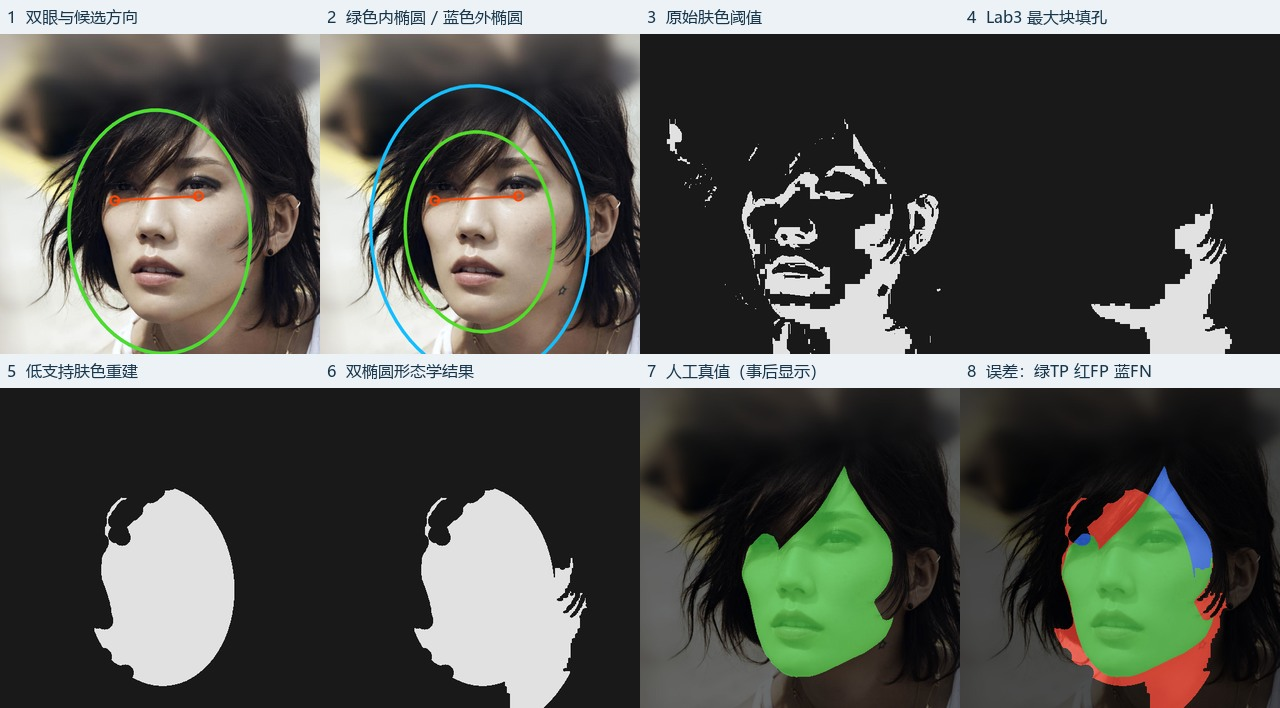
\includegraphics[width=0.98\textwidth]{lab4_dual_00660.jpg}
\caption{验证图 00660 的低支持度放宽阈值重建对照。Lab3 仅检出脖颈与下颌局部（F1 0.2064），双椭圆引导的低支持重建将面部主体完整找回，F1 提升至 0.8031。}
\label{fig:lab4_dual_00660}
\end{figure}

最后，实验四方案的四项方法边界与局限在于：（1）82.89\% 全局 F1 是在 32 张验证图上经过多轮开发迭代得到的结果，不能直接等同于未见测试集上的无偏泛化性能；（2）双眼定位在很大程度上依赖训练集统计出的左右眼居中窗口先验；（3）在暖调头发样本上，$k_{\text{rec}}=2.00$ 放宽阈值仍可能将内椭圆上缘的刘海纳入重建区域；（4）仅有的两张微降样本（00712 与 00731）因过渡带弱闭运算连接少量边缘像素产生约 $-0.001\sim-0.002$ 的极小波动。
